\section{Выбор схемы усилителя переменного тока}

\subsection{Построение усилителя на основе инвертирующего решающего усилителя (РУ)}

\begin{figure}[H]
	\centering
	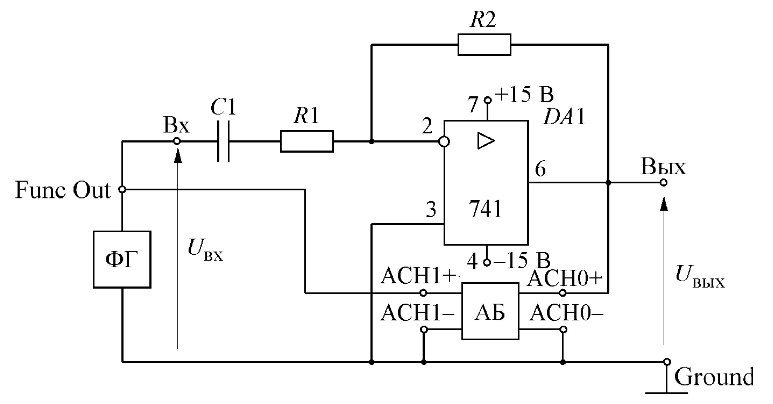
\includegraphics[width=0.7\linewidth]{photo/invertring_py}
	\caption{Схема инвертирующего РУ с разделительным конденсатором на входе}
	\label{fig:invertring_py}
\end{figure}

Коэффициент усиления и входное сопротивление УПТ
(рис.~\ref{fig:invertring_py}) в полосе пропускания определяются схемными 
функциями инвертирующего РУ:

$$ 
K_{UИ} = \dfrac{U_{вых}}{U_{вх}} \approx -\dfrac{R_2}{R_1}; 
R_{вх. и} = \dfrac{U_{вх}}{I_{вх}} \approx R_1
$$

Учитывая значения параметров, заданные техническим заданием 
$ K_U = 1000 $ и $ R_{вх} = 200~кОм $ 
получим:

$ R_1 = 200 кОм $

$ R_2 = K_U R_1 = 1000 \times 200 = 200~МОм $

Так как по результатам расчета схемы на 
рис.~\ref{fig:invertring_py}
$ R_2 = 200~МОм \gg 10~МОм $,
считаем, что такая схема не подходит 
и дальше исследовать её далее не нужно.

\subsection{Схемная реализация усилителя на базе неинвернтирующего РУ}

\begin{figure}[H]
	\centering
	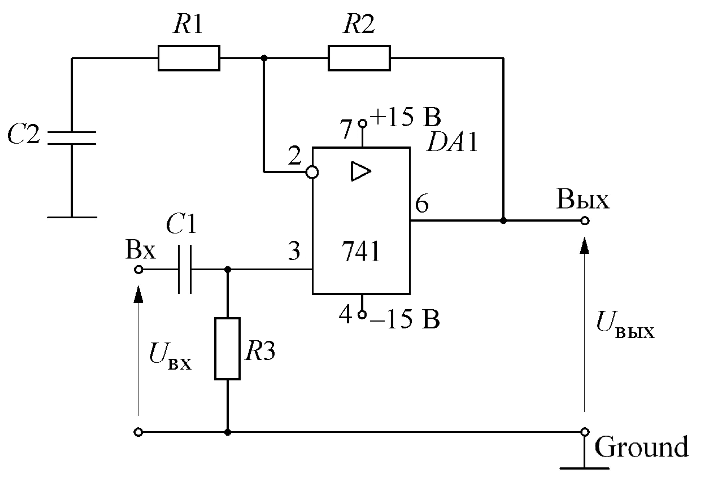
\includegraphics[width=0.7\linewidth]{photo/non_inverting_py}
	\caption{Схема усилителя переменного тока на базе неинвертирующего РУ}
	\label{fig:non_invertring_py}
\end{figure}

Коэффициент усиления и 
входное сопротивление 
усилителя переменного тока в полосе пропускания 
определяются схемными функциями неинвертирующего РУ 
(сопротивлением конденсаторов С1 и С2 в полосе пропускания 
в первом приближении можно пренебречь):

$$
K_{Uни} = \dfrac{U_{вых}}{U_{вх}} \approx 1 + \dfrac{R_2}{R_1};
R_{вх. ни} = \dfrac{U_{вх}}{I_{вх}} \approx R_3
$$

Примем $ R_{вх. ни} \approx R_3 = 200~кОм $\\

Примем ёмкость конденсаторов $ C_1 = C_2 = 1~мкФ $\\

$ f_н = \dfrac{1}{2 \pi R_1 C_2} $\\

Учитывая, что согласно ТЗ $ f_н = 200~Гц $, найдём $ R_1 $ и $ R_2 $:\\

$ R_1 = \dfrac{1}{2 \pi C_1 f_н} = \dfrac{1}{6.28 * 1 * 10^{-6} * 200} = 796.178~Ом $\\

$ R_2 = R_1 (K_U - 1) = 796.178 * 999 = 795.382~кОм $\\

Далее найдём граничную частоту ОУ:\\

$ f_{ср} = |K_U| f_в = |1000| * 20 * 103 = 20000~кГц = 20~МГц  $\\

Отметим, что такой усилитель подобрать достаточно сложно. 
Возможно, что усилитель (рис.~\ref{fig:non_invertring_py}) 
будет иметь малую граничную частоту $ f_в $, 
меньше чем в техническом задании
($ f_в = 20~кГц $) потому что усиления усилителя реализуются 
на одной усилительной подсхеме, 
проверить это можно только в системе \textit{Multisim}. 
По рассчитанным данным схема подходит, 
но сделать окончательное суждение допустимо после её построения 
в системе \textit{Multisim} и проверки $ f_в $ 
на соответствие входным данным.

\subsection{Построение усилителя на основе двух усилительных подсхем}

\begin{figure}[H]
	\centering
	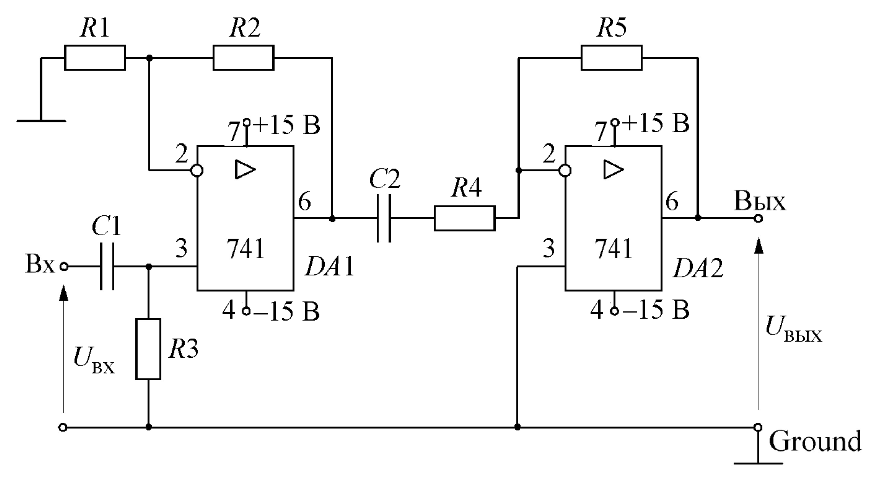
\includegraphics[width=0.7\linewidth]{photo/sub2_py}
	\caption{Схема усилителя переменного тока}
	\label{fig:sub2_py}
\end{figure}

От недостатка усилителя на рис.~\ref{fig:non_invertring_py} 
свободна схема усилителя переменного тока, 
представленная на рис.~\ref{fig:sub2_py}. 
Этот усилитель состоит из двух усилительных подсхем: 
входная подсхема реализуется на неинвертирующем РУ $ (DA_1; R_1; R_2; R_3; С_1) $, 
что позволяет обеспечить большое входное сопротивление усилителя переменного тока; 
выходная подсхема представляет собой инвертирующий РУ ($ DA_2; R_4; R_5; С_2 $) 
и используется для получения высокого коэффициента усиления $ K_U $ всего усилителя. 
В полосе пропускания

$$ 
K_U = 
K_{Uи} K_{Uни} = 
\left( 1 + \dfrac{R_2}{R_1} \right)
\left( -\dfrac{R_2}{R_1} \right) 
$$

Примем ёмкость конденсаторов $ C_1 = C_2 = 1~мкФ $\\

Нижняя граница частоты полосы пропускания 
усилителя переменного тока (рис.~\ref{fig:sub2_py}) 
определяется соотношением:

$ f_н = \dfrac{1}{2 \pi R_4 C_2} $\\

Учитывая, что согласно ТЗ $ f_н = 200~Гц $, найдём $ R_2 $:\\

$ R_2 = \dfrac{1}{2 \pi C_2 f_н} = \dfrac{1}{6.28 * 1 * 10^{-6} * 200} = 796.178~Ом $\\

Так как необходимо распределить коэффициент усиления на две усилительные подсхемы: 

$ K_{Uи} = K_{Uни} = \sqrt{K_{U}} = \sqrt{1000} = 31.623 $\\

$ R_{вх} = R_3 = 200~кОм $ (для обеспечения сопротивления 200~кОм)\\

Принимаем $ R_1 = 1~кОм $\\

$ R_2 = R_1 (\sqrt{K_U} - 1) = 1 * (31.623 - 1) = 30.623 $\\

$ R_5 = K_{Uи} R_4 = 31.623 * 0.796 = 25.172~кОм $\\

Далее находим граничную частоту операционного усилителя:\\

$ f_{ср} = |K_U| f_в = |31.623| * 20 * 10^3 = 632,46 кГц $\\

По рассчитанным данным схема подходит, 
но сделать окончательное суждение допустимо 
после её построения в системе \textit{Multisim}.

\subsection*{Общий вывод по выбору схемы}
\addcontentsline{toc}{subsection}{Общий вывод по выбору схемы}

В ходе проекта было рассмотрено 
три варианта схем усилителя переменного тока, 
реализующих параметры, заданные заданием – 
однокаскадный инвертирующий усилитель, 
однокаскадный неинвертирующий усилитель и 
двухкаскадный усилитель.

Так как согласно заданию 
требуется высокий коэффициент усиления (1000)
и одновременно большое входное сопротивление (200~КОм), 
то оказалось, что схема инвертирующего усилителя 
принципиально не подходит – 
сопротивление в цепи обратной связи получается большим
и не реализуемым на практике.
Вторая схема реализуема на практике, однако, 
как показали расчеты, требует усилителя 
с большой граничной частотой.

Такие усилители, как правило, 
обладают невысокой нагрузочной способностью. 
А по заданию необходимо 10~мА.
Оптимальной для реализации оказалась третья схема. 
Как показали расчеты, в ней допустимо использовать
усилители  с граничной частотой 2~МГц. 
Это связано с тем, что коэффициент усиления 
каждого каскада невысок. 
У обоих каскадов был обеспечен одинаковый 
(сравнительно небольшой) коэффициент усиления,
как и требовалось в задании.



